
\Section{Payment channels}
A payment channel is a channel where transactions can be exchanged trustlessly on channels other than directly on the blockchain.
This is what is usually referred to as off-chain transactions.
In their most naive form a payment channel can simply be Alice and Bob exchanging promises of future transactions later.
This however is not trustless and any of the parties could later withdraw from the promise without punishment (other than maybe loss of friendship and future trust).

To build a trustless payment channel there are several ways to go about as Script is quite versatile.
The method that will be covered here uses a type of channel \textbf{funding transaction that requires the signature from both parties to spend}, and the channel balance is updated via special commitment transactions that spend the funding output. Each party in the channel has their own version of the commitment transaction. Whenever a commitment transaction is broadcast to the blockchain the channel is closed as the funding transaction can't be spent twice. To update the balance in the channel both parties create new commitment transactions and signs the other parties commitment transaction.\cite{lightningnetwork_2019}\cite{antonopoulos_2017}
Let's take a look at a naive example:

\Subsubsection{The naive payment channel}
Imagine Alice and Bob wants to open a payment channel between each other. They create a funding transaction and the initial commitment transactions. Let's say they both funded the channel with 1 Bitcoin each. The initial commitment transactions would then have one output paying 1 Bitcoin to Alice and one output paying 1 Bitcoin to Bob, let's call this commit (\textbf{C0}).
The funding transaction is broadcast to the blockchain.

A bit later Alice buys one funny hat from Bob for 0.1 Bitcoins. To complete the transaction they create two new commitment transaction that pays 0.9 Bitcoin to Alice and 1.1 Bitcoin to Bob and signs them for each other, let's call this new commitment (\textbf{C1}). Any number of transactions could be exchanged this way. The channel could be closed by any one broadcasting their commitment transaction. This naive implementation of a payment channel has a fatal flaw however. 

A payment channel needs some safety measures to be safe from malicious actors. The above example lacks a mechanism for preventing old commitment transactions from making their way into the blockchain and still paying the malicious party.. For example after the initial funny hat transaction above (\textbf{C1}) Alice could just broadcast the initial commit transaction (\textbf{C0}) and reclaim the 0.1 Bitcoins she spent. Bob would have no way of preventing this in this naive implementation.

\Subsubsection{Transaction flow diagrams}
The transactions that are involved in making payment channels grows larger the more features that are added. To make it easier to understand, diagrams are used together with the descriptions. In Figure \ref{fig:anatomy} a basic overview of the diagram-realm transaction is shown. Lines leading from outputs to inputs means that the connected input are spending that output. Note that one output can be connected to several inputs but each input can only be connected to one output, of course an output can only be spent once, this will be clarified later. A question mark (\textbf{?}) in the broadcaster field indicates either that the sender is unknown or that who sends it is irrelevant. 


\begin{figure}[H]
	\centering
	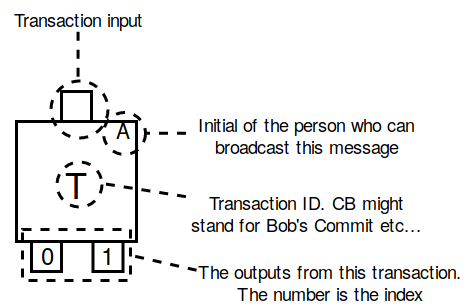
\includegraphics[width=0.5\textwidth]{background/images/tx_anatomy.png}
	\caption{Different parts of a transaction as they appear in diagrams.}
	\label{fig:anatomy}
\end{figure}

\Subsubsection{Payment channel with breach remedy}\label{breach_remedy}
To prevent old transactions from being sent to the blockchain a new mechanism needs to be devised. This can be done via something called revocable delivery and breach remedy (Some times called just revocation).
Instead of both parties holding the same commit. They each get an individual one that differs in it's outputs. 

\begin{figure}[H]
	\centering
	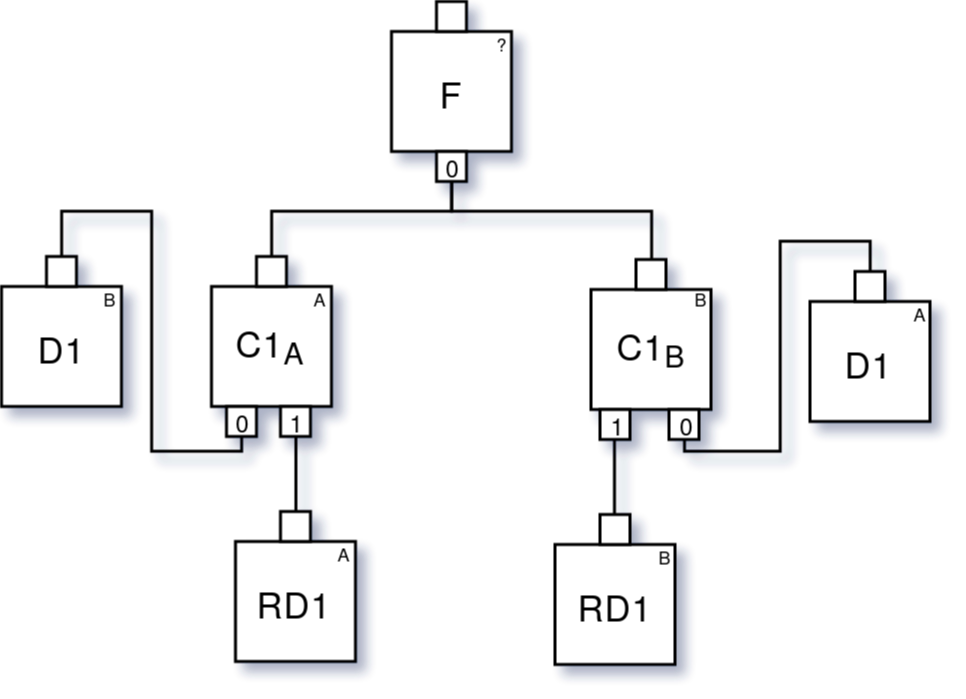
\includegraphics[width=0.6\textwidth]{background/images/payment_channel_pre_breach.png}
	\caption{Payment channel, with commits using revocable delivery mechanism}
	\label{fig:pre-breach}
\end{figure}

Figure \ref{fig:pre-breach} shows how the payment channel appears after the first commitment transactions has been made. Let's say the channel is between Alice (A) and Bob (B) and the balance in the channel is 0.5 BTC for Alice and 0.5 BTC for Bob. 

Lets' take a look at the left side of this diagram. \textbf{$C1_{A}$} is the commitment transaction on Alice's side of the channel. As with all commitment transactions it spends the funding transaction. It has two outputs. Output 0 sends 0.5 BTC to Bob completely unencumbered. Output 1 is a bit more complicated however. It pays into a revocable delivery contract worth 0.5 BTC.\footnote{The contract is a script, and it's payed to via P2SH} The contract is constructed with a relative time lock that allows Alice to claim her share of the money after x amount of time (relative to the broadcast time of $C1_{A}$, often described in terms of blocks) or pays to whomever can sign using the pre-generated revocation keys (See section \ref{homomorphism})

D1 is the transaction Bob uses to claim his money in case Alice decides to broadcast her commitment transaction ($C1_{A}$).

RD1 is the transaction that Alice uses to claim her money. The transaction has a relative timelock on it that makes it so it can't be broadcast until x blocks has passed since $C1_{A}$ was included in the blockchain. \textbf{From now on the relative timelock will be 100 blocks in all the following examples}.

The right side is identical, only that the RD1 and D1 relationship is reversed, meaning that Alice can claim her money directly and Bob has to wait. 

If Alice wants to send 0.1 BTC to Bob they need to update the channel with new commitment transactions and then invalidate the old transaction. The transaction diagram will now look like figure \ref{fig:pc-update}

\begin{figure}[H]
	\centering
	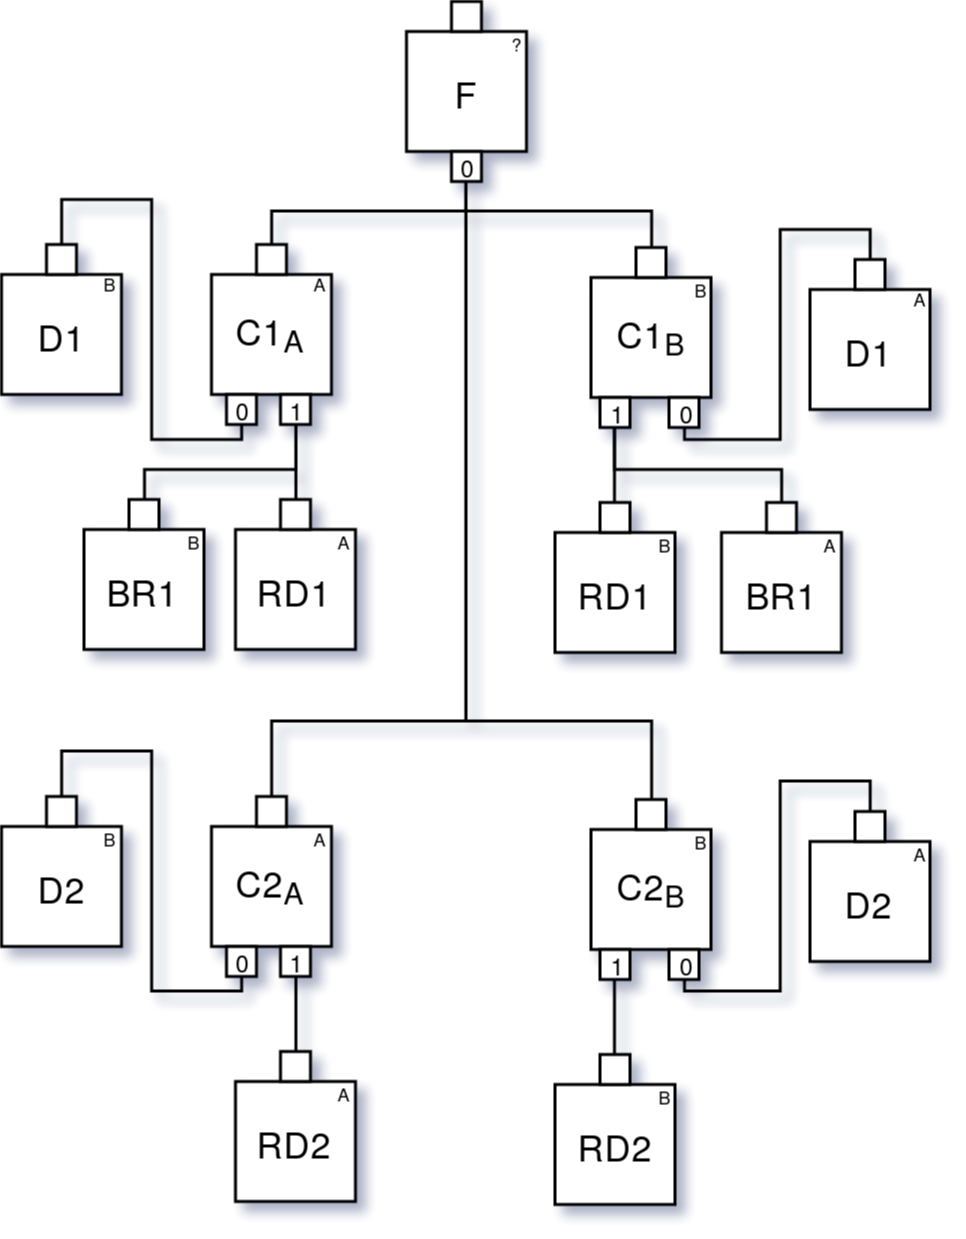
\includegraphics[width=0.65\textwidth]{background/images/payment_channel_updated.png}
	\caption{Updated payment channel, with breach remedies for old commitment transactions}
	\label{fig:pc-update}
\end{figure}

Figure \ref{fig:pc-update} shows the state of the channel after the new commitment transactions have been finalized. 
$C2_{A}$ is a lot like the previous commitment transaction with a few changes. The primary change is of course the channel balance, output 0 now has 0.6 BTC as value and output 1 has 0.4 BTC (Because Alice sent 0.1 BTC to Bob).

Another important update to the channel is the breach remedy. BR1 is the breach remedy for the first commitment transaction, it's purpose is to prevent old commitment transactions from being broadcast.\cite{lightningnetwork_2019} The breach remedy can be created after Alice has revealed the secret private key she used when creating the revocation key. Of course to prevent a new false breach remedy to be created for $C2_{A}$ Alice uses a new revocation key for all new commitment transactions. If Alice tries to take back her money by broadcasting an old commitment transaction Bob can prevent it by broadcasting the breach remedy, this is possible because of the timelock on Alice's claim being time-locked.\cite{lightningnetwork_2019}

These are the steps taken whenever someone wants to send money in the channel (Under the assumption that commitment n-1 ($C_{n-1}$) was the latest commitment transaction in the channel), Alice is assumed to be the sender:\\\\
%\begin{enumerate}
	\textbf{1.} Both parties create new revocation public keys.\\
	\textbf{2.} Alice creates the commitment on Bob's side ($Cn_{b}$) using the revocation key from the previous step, signs it and sends it to Bob.\\
	\textbf{3.} Bob creates the commitment on Alice's side ($Cn_{a}$) using the revocation key from the previous step, signs it and sends it to Alice.\\
	\textbf{4.} Each party generates their respective Delivery and Revocable delivery transactions (Dn and BRn)\\
	\textbf{5.} Both parties reveal the secret used to create the revocation keys for the previous commitment transactions ($C_{n-1}$)\\
	\textbf{6.} From these revocation keys each party constructs the breach remedy ($BR_{n-1}$) for the previous commitment on the other persons side.\\
%\end{enumerate}

These steps can be repeated however many times until the channel is closed. 

